\section{Results}
In this section, we will present verification results for implementation and the Beta algorithm for two modes of concurrency. The first mode of concurrency is asynchrony which is the intended mode for the Beta algorithm. The second implementation is synchronized to investigate the influence of the concurrency mode on algorithm properties. In the asynchronous case, presented in Figure \ref{fig:implementation}, robots can move at different rates. Each robot is forced to move from \texttt{forward} location after \texttt{T\_MAX} amount of time but can also transition sooner. In the synchronized implementation, presented in Figures \ref{fig:implementation_synchronised} and \ref{fig:implementation_synchronised_barrier}, all robots are forced to move at the same time by the synchronization mechanism.



\subsection{Verification of asynchronous implementation}
% System specification
\begin{figure}[H]
\caption{System specification for asynchronous implementation}
\label{fig:implementation_asynchronous_system}
\begin{lstlisting}[style=code]
N = 2;      // Number of robots
R = 1;      // Signal radius
STEP = 1;   // Step size
BETA = 1;   // Beta parameter
G = 3;      // Grid boundary
T_MAX = 1;  // Time threshold
\end{lstlisting}
\end{figure}

% Properties
\begin{figure}[H]
\caption{Successfully verified properties for synchronous implementation}
\label{fig:implementation_asynchronous_properties}
\begin{lstlisting}[style=code]
1.  A[] forall(i : int[0, N-1]) x[i] != G or y[i] != G
2.  A[] forall(i : int[0, N-1]) abs(x[i]) <= G && abs(y[i]) <= G
3.  E<> C > 0 && P0.turn_random
4.  E<> C > 0 && P0.turn_180
5.  A[] P0.forward imply P0.t <= T_MAX
6.  E<> P0.turn_180 && not gridBoundary(0)
7.  E<> P0.turn_180 && gridBoundary(0)
8.  E<> P0.forward && not turnRandom(0) && not turn180(0)
9.  A[] P0.t != 0 imply P0.forward
10. A[] (P0.turn_random or P0.turn_180 or P0.grid or P0.grid or P0.if or P0.else_if) imply P0.t == 0
11. A[] forall(i : int[0, N-1]) shared_neighbours[i][0] == 0 and shared_neighbours[i][1] == 0
12. A[] forall(i : int[0, N-1]) C < 0 imply k[i] == N-1
13. A[] forall(i : int[0, N-1]) C > 0 imply x_dir[i] != 0 or y_dir[i] != 0
14. A[] not deadlock
\end{lstlisting}    
\end{figure}

% Explanation of properties
\noindent
Explanation of properties from Figure \ref{fig:implementation_asynchronous_properties}:\\
1. For all the paths through the system, no robot can have their x and y coordinates equal to the grid boundary at the same time. No robot will ever reach the corner of the grid.\\
2. For all the paths through the system, all robots will stay within the grid boundaries.\\
3. There exists a path through the system, for a robot to reach location \texttt{turn\_random} after initialization. This means that following locations are reachable: \texttt{forward}, \texttt{grid}, \texttt{if}, \texttt{else\_if}. It also means that following transitions are reachable: \texttt{turn\_random} $\rightarrow$ \texttt{forward}, \texttt{forward}n $\rightarrow$ \texttt{grid}, \texttt{grid} $\rightarrow$ \texttt{if}, \texttt{if} $\rightarrow$ \texttt{else\_if}, \texttt{else\_if} $\rightarrow$ \texttt{turn\_random}.\\ 
4. There exists a path through the system, for a robot to reach location \texttt{turn\_180} after initialization.\\
5. For all the paths through the system, a robot will obey the invariant on location \texttt{forward}.\\
6. There exists a path through the system, for a robot to reach location \texttt{turn\_180} without reaching the boundary of the grid. This means that transition from \texttt{if} to \texttt{turn\_180} is reachable.\\
7. There exists a path through the system, for a robot to reach location \texttt{turn\_180} as a result of reaching the boundary of the grid. This means that transition from \texttt{grid} to \texttt{turn\_180} is reachable.\\
8. There exists a path through the system, for a robot to reach location \texttt{forward} without changing its direction. \\
9. For all the paths through the system, robot's clock value different than zero implies it being in the \texttt{forward} location. This means that time perceived by the robot is only allowed to pass in the \texttt{forward} location.\\
10. For all the paths through the system, a robot's presence in the listed location imply that its clock value is equal to zero. For the robot, time will not pass in any other location than forward.\\
11. For all the paths through the system, two robots will not share a neighbor. This is a consequence of a fact that in the system consisting of two robots, they cannot have a neighbor in common.\\
12. For all paths through the system, all robots are fully connected as part of system initialization.\\
13. For all paths through the system, all robots have their directions set after system initialization.\\
14. There is no path through the system, which will result in deadlock.\\



\subsection{Verification of synchronized implementation}
% System specification
\begin{figure}[H]
\caption{System specification for synchronized implementation}
\label{fig:implementation_synchronised_system}
\begin{lstlisting}[style=code]
N = 2;      // Number of robots
R = 2;      // Signal radius
STEP = 1;   // Step size
BETA = 1;   // Beta parameter
G = 3;      // Grid boundary
\end{lstlisting}
\end{figure}

% Properties
\begin{figure}[H]
\caption{Successfully verified properties for synchronized implementation}
\label{fig:implementation_synchronised_properties}
\begin{lstlisting}[style=code]
1.  A[] forall(i : int[0, N-1]) x[i] != G or y[i] != G
2.  A[] forall(i : int[0, N-1]) abs(x[i]) <= G && abs(y[i]) <= G
3.  E<> (x[0] != 0 or y[0] != 0) and P0.turn_random
4.  A[] (P0.forward and P1.forward) imply C0.n == 0
5.  A[] C0.n == N imply not (P0.forward or P1.forward)
6.  E<> P0.turn_180 && not gridBoundary(0)
7.  E<> P0.turn_180 && gridBoundary(0)
8.  E<> P0.forward && not turnRandom(0) && not turn180(0)
9.  A[] P0.turn_180 imply (P1.forward or P1.grid)
10. A[] forall(i : int[0, N-1]) shared_neighbours[i][0] == 0 and shared_neighbours[i][1] == 0
11. A[] forall(i : int[0, N-1]) (x_dir[i] == 0 and y_dir[i] == 0) imply k[i] == N-1
12. A[] not deadlock
\end{lstlisting}    
\end{figure}

% Explanataion of properties
\noindent
Explanation of properties from Figure \ref{fig:implementation_synchronised_properties}:\\
1. For all the paths through the system, no robot can have their x and y coordinates equal to the grid boundary at the same time. No robot will ever reach the corner of the grid.\\
2. For all the paths through the system, all robots will stay within the grid boundaries.\\
3. There exists a path through the system, for a robot to reach location \texttt{turn\_random} not only as a result of initialization. This means that following locations are reachable: \texttt{forward}, \texttt{grid}, \texttt{if}, \texttt{else\_if}. It also means that following transitions are reachable: \texttt{turn\_random} $\rightarrow$ \texttt{forward}, \texttt{forward} $\rightarrow$ \texttt{grid}, \texttt{grid} $\rightarrow$ \texttt{if}, \texttt{if} $\rightarrow$ \texttt{else\_if}, \texttt{else\_if} $\rightarrow$ \texttt{turn\_random}. This property is false for a system with signal radius equal to 1.\\ 
4. For all the paths through the system, if both robots are in the \texttt{forward} location, then the value of the synchronization mechanism must be equal to 0.
5. For all the paths through the system, if value of synchronization mechanism is equal to the number of robots in the system, none of the robots can be in the \texttt{forward} location.
6. There exists a path through the system, for a robot to reach location \texttt{turn\_180} without reaching the boundary of the grid. This means that transition from \texttt{if} to \texttt{turn\_180} is reachable.\\
7. There exists a path through the system, for a robot to reach location \texttt{turn\_180} as a result of reaching the boundary of the grid. This means 
8. There exists a path through the system, for a robot to reach location \texttt{forward} without changing its direction.\\
9. For all the paths through the system, if the first robot is in the \texttt{turn\_180} location, the other has to be in either \texttt{forward} or \texttt{grid} location. More generally, only one robot can be changing its direction at any given time.\\ 
10. For all the paths through the system, two robots will not share a neighbor. This is a consequence of a fact that in the system consisting of two robots, they cannot have a neighbor in common.\\
11. For all paths through the system, if none of the robots have their direction set they must be fully connected to other robots. This property aims to check the correctness of initialization. \\
12. There is no path through the system, which will result in deadlock.\\



\subsection{Verification of Beta algorithm - asynchronous implementation}
% System specification
\begin{figure}[H]
\caption{System specification for synchronized implementation}
\label{fig:algorithm_asynchronous_system}
\begin{lstlisting}[style=code]
N = 3;      // Number of robots
R = 1;      // Signal radius
STEP = 1;   // Step size
BETA = 2;   // Beta parameter
G = 3;      // Grid boundary
\end{lstlisting}
\end{figure}

% Properties
\begin{figure}[H]
\caption{Successfully verified properties for Beta algorithm, for system specification defined in Figure \ref{fig:algorithm_asynchronous_system}}
\label{fig:algorithm_asynchronous_properties}
\begin{lstlisting}[style=code]
1. E<> exists(i : int[0, N-1]) k[i] == 0 and last_k[i] == 0
2. E<> forall(i : int[0, N-1]) k[i] == 0 and last_k[i] == 0
3. E<> forall(i : int[0, N-1]) C < T_MAX and k[i] == 0 and last_k[i] == 0 
\end{lstlisting}    
\end{figure}

% System specification
\begin{figure}[H]
\caption{System specification for synchronized implementation}
\label{fig:algorithm_asynchronous_system_2}
\begin{lstlisting}[style=code]
N = 4;      // Number of robots
R = 1;      // Signal radius
STEP = 1;   // Step size
BETA = 2;   // Beta parameter
G = 3;      // Grid boundary
\end{lstlisting}
\end{figure}

% Properties
\begin{figure}[H]
\caption{Successfully verified properties for Beta algorithm, for system specification defined in Figure \ref{fig:algorithm_asynchronous_system_2}}
\label{fig:algorithm_asynchronous_properties_2}
\begin{lstlisting}[style=code]
1. E<> exists(i : int[0, N-1]) k[i] == 0 and last_k[i] == 0
\end{lstlisting}    
\end{figure}

\noindent
Explanation of properties for Figure \ref{fig:algorithm_asynchronous_properties} and Figure \ref{fig:algorithm_asynchronous_properties_2}:\\
1. There exists a path through the system, for a robot to become disconnected for at least two steps.\\
2. There exists a path through the system, where all robots become disconnected for at least two steps.\\
3. There exists a path through the system, where all robots become disconnected for at least two steps with global time of the system not exceeding a time threshold used for invariants.\\
\\
Property defined in Figure \ref{fig:algorithm_asynchronous_properties_2} was successfully verified for the system consisting of four robots. UPPAAL generated a diagnostic trace that is a path through the system satisfying the property. It presents a scenario where a single robot gets disconnected for at least two steps. This trace will be used as a starting point to show possible scenarios. In the positive scenario, presented in Figure \ref{fig:reconnection}, a disconnected robot is reconnected with the swarm. In the negative scenario, presented in Figure \ref{fig:lost_connection}, a disconnected robot fails to reconnect with the swarm and may reconnect in the future only due to limited grid area. All the presented scenarios exceeding the trace were obtained using UPPAAL's symbolic simulator, therefore presented states of the system are reachable.\\
\\
Diagrams present robot swarm system states. The state of the system is represented by robots placed on the two-dimensional grid. A grid is a square with a side of length equal to six. The grid center serves as the origin of the coordinate system. A robot is represented by its position on the grid marked with a dot, direction indicated by an arrow, signal radius visualized by a circle. Numbers inside of the circle indicate a number of robots in a given location. There might be multiple system states in between those presented in the diagram however, they are not crucial for illustrative purposes. States marked with the letter T are part of the trace generated while verifying property from Figure \ref{fig:algorithm_asynchronous_properties_2}.
\newpage
\noindent
The scenario described by the diagnostic trace starts with all robots placed in the origin of the coordinate system and without a set direction. Then each robot gets its direction set before moving forward for the first time. The basis for this textual description is the implementation of the Beta algorithm presented in Figure \ref{fig:implementation}. In the diagnostic trace, one robot has its direction set to 'right' while the other three robots have their direction set to 'up'. After the robot moves one step to the right it updates its connection information. It is connected to all of the robots as they are within the reach of its signal. Other robots move up and update their connection information. All of the robots react to the loss of the robot that moved to the right and perform 180 degree turn to change their direction. The robot that moved to the right did not update its connection information and perceives itself as fully connected to other robots. It continues to move to the right, updates its connection information and as a consequence performs a 180 degree turn.\\
\\
\noindent
Figure \ref{fig:reconnection} presents diagnostic trace marked with T and one of possible positive scenarios marked with R. In the positive scenario the robot that was moving to the right, performs a 180 degree turn and reconnects with a swarm by moving left. All robots are within their signal range. Another positive scenario could involve one of three robots traveling to the center of the grid to serve as a bridge between the robot that moved to the right and two other robots that moved up.

\begin{figure}[H]
\caption{Trace and reconnection}
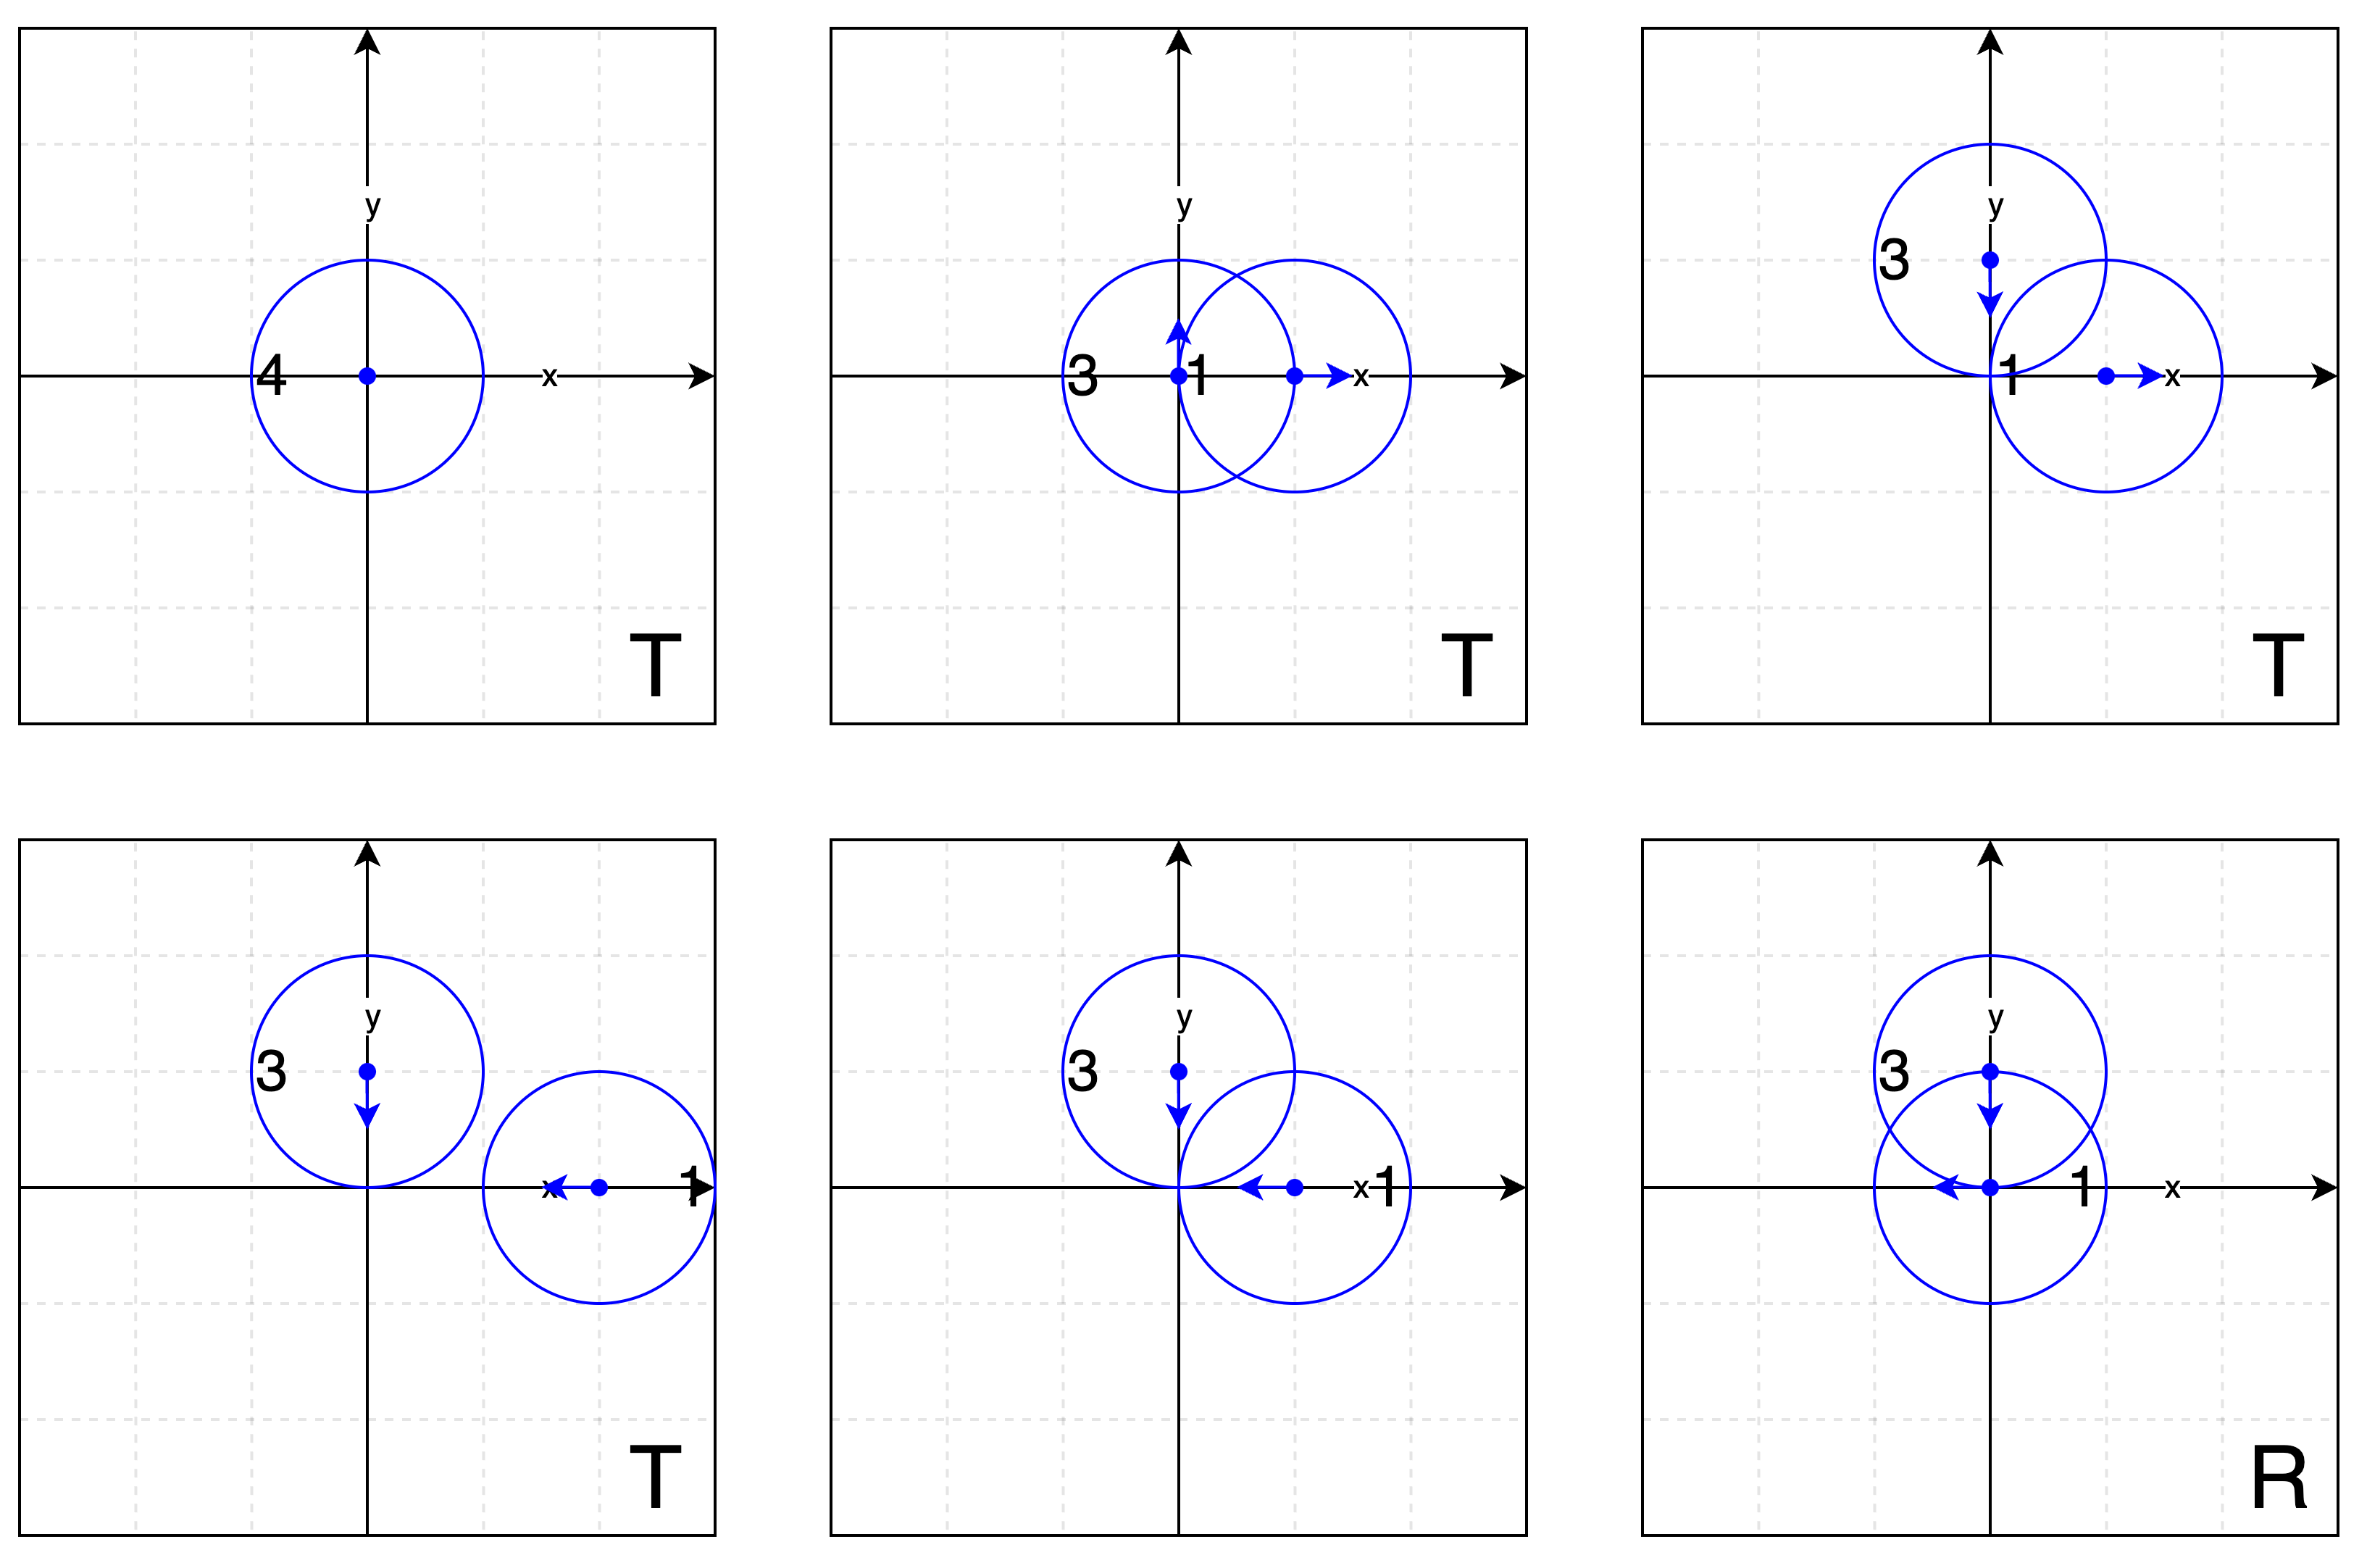
\includegraphics[width=\textwidth]{images/reconnection.png}
\label{fig:reconnection}
\end{figure}
\newpage
\noindent
Figure \ref{fig:lost_connection} presents a diagnostic trace marked with T, a lost connection scenario marked with L, and the scenario of reconnection due to the grid boundary marked with B. Because the robots move asynchronously, it is possible for three robots that initially moved up to move down before the other robot makes a single move toward the center. This behavior is shown in the middle row of the diagram. After that, the robot that was on the right would traverse to the left side. If the grid was not limited, the robot would become disconnected forever, which is shown in the L scenario. Because the grid is limited and robots will perform 180 degree turn it is possible for them to reconnect as the result of reaching the boundary, which is shown in the B scenario.

\begin{figure}[H]
\caption{Trace and lost connection}
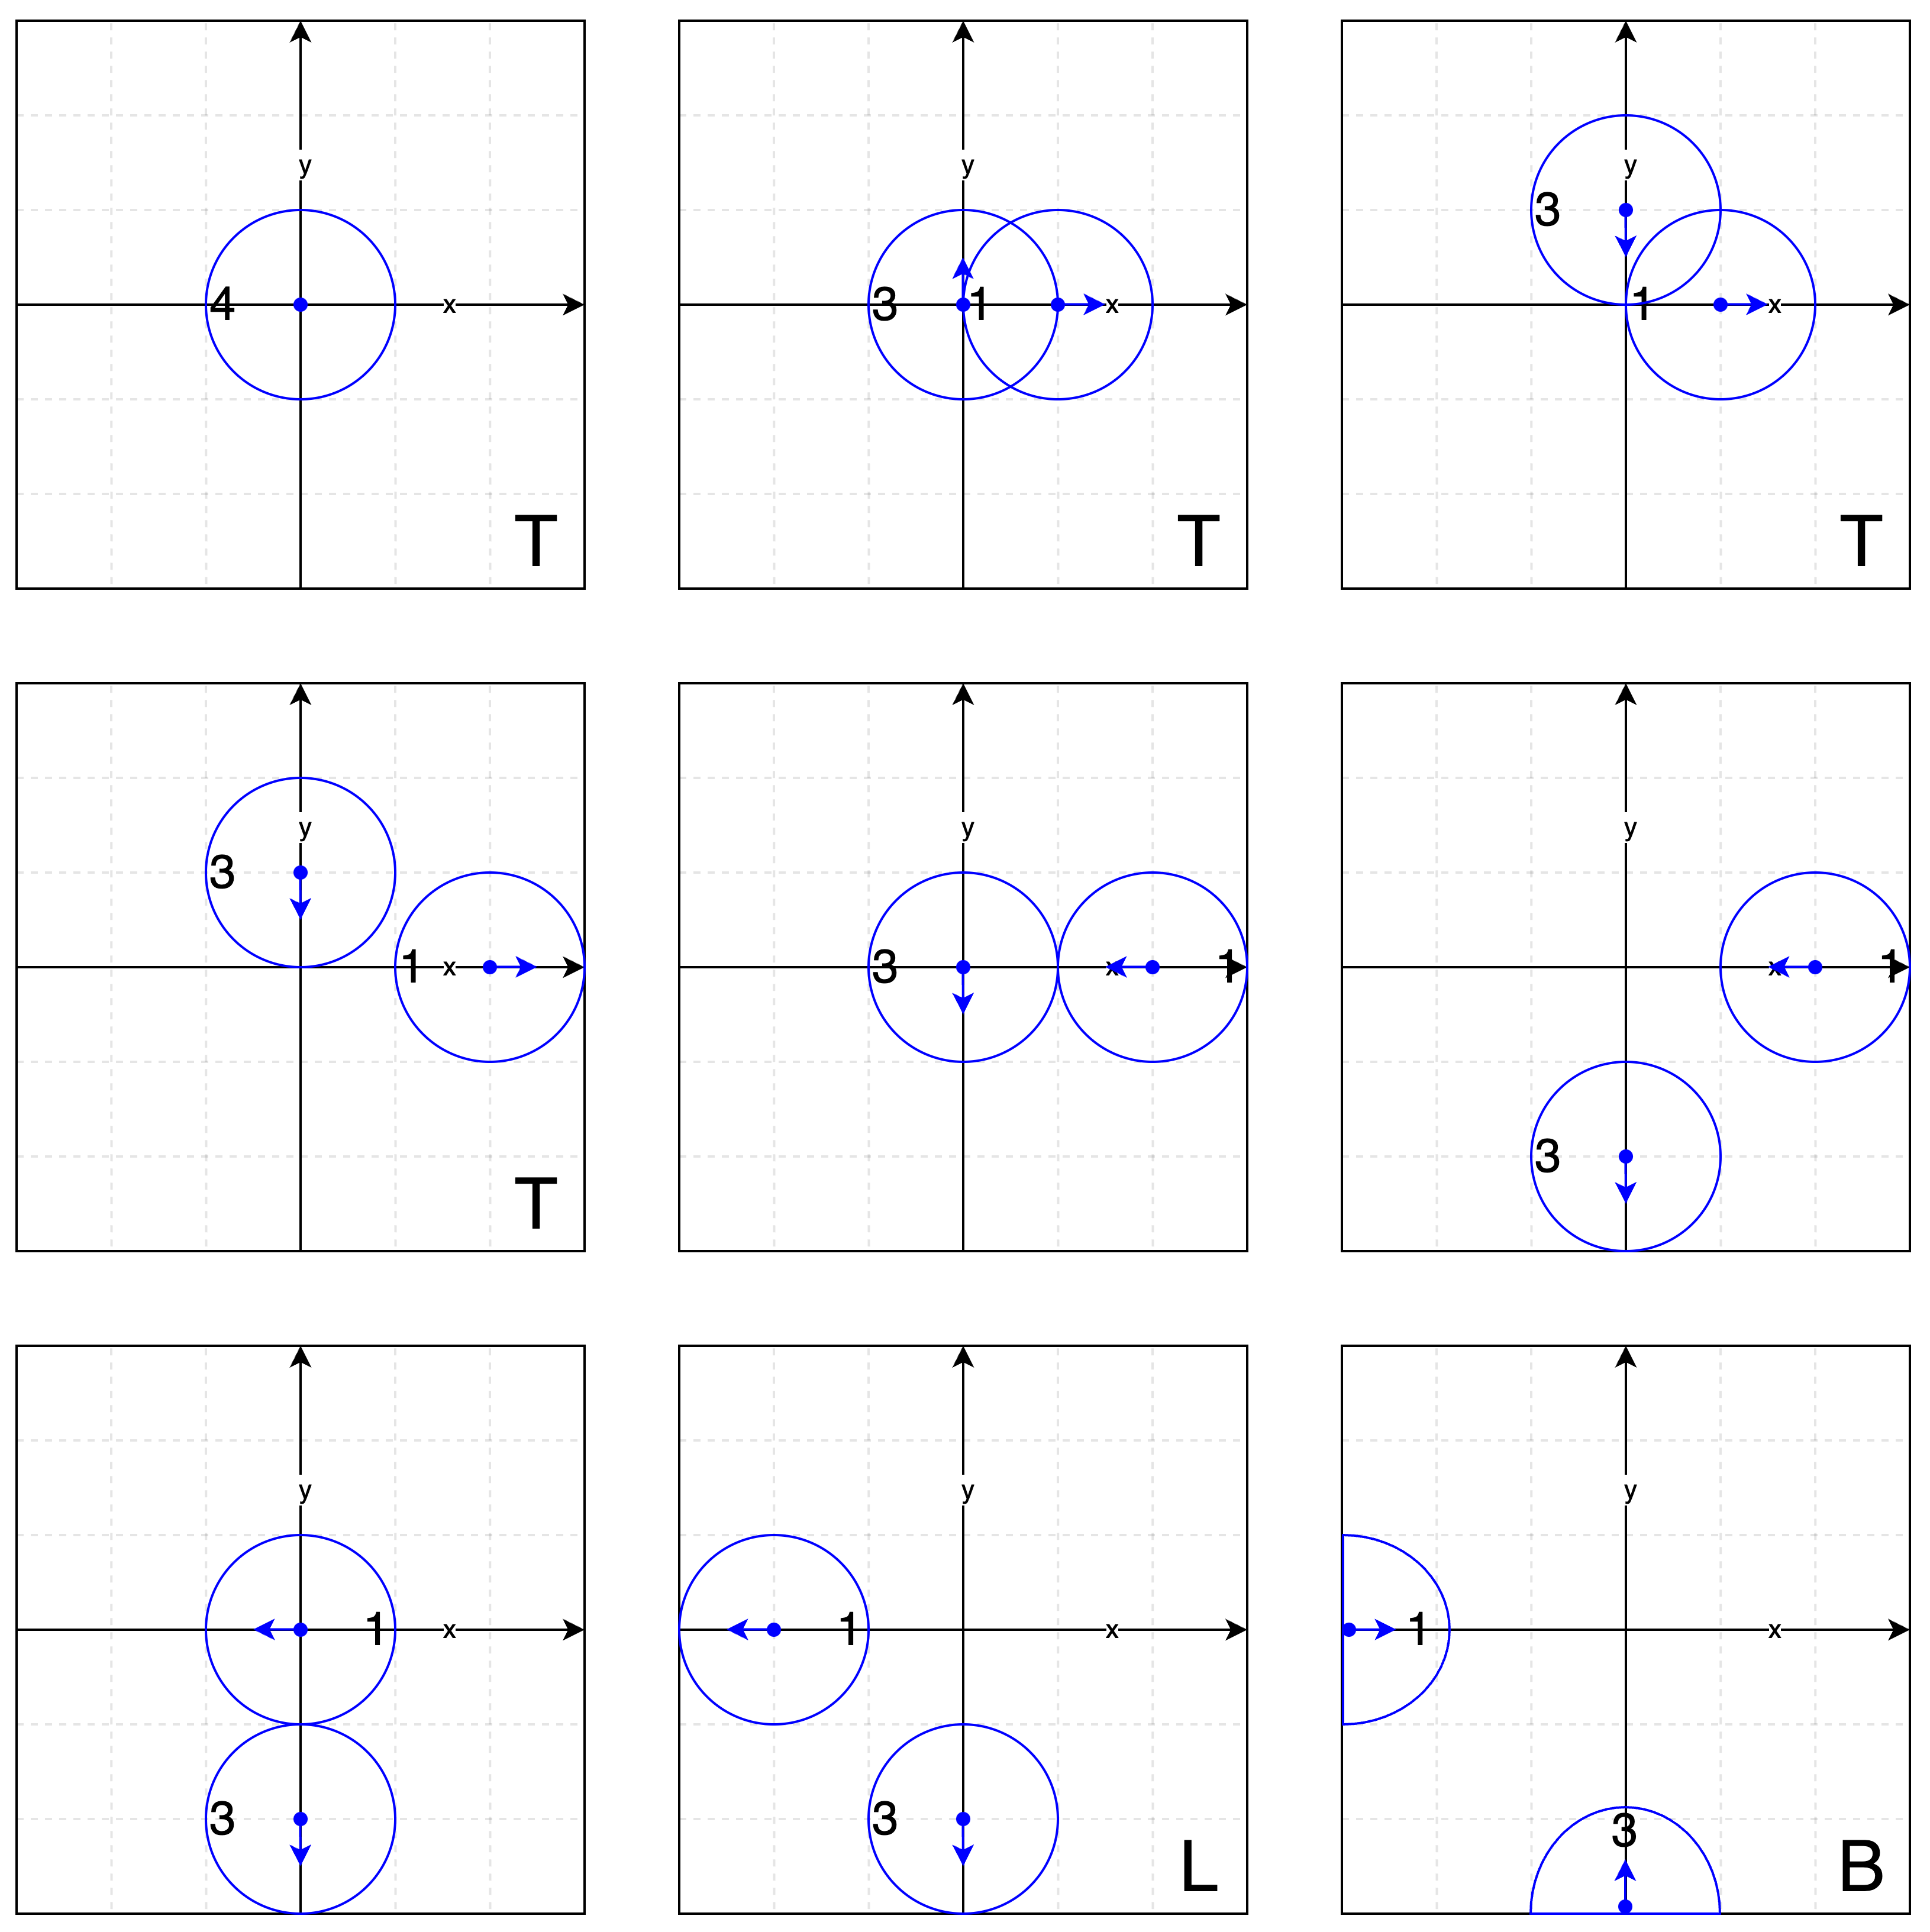
\includegraphics[width=\textwidth]{images/lost_connection.png}
\label{fig:lost_connection}
\end{figure}


\subsection{Verification of Beta algorithm - synchronized implementation}
% System specification
\begin{figure}[H]
\caption{System specification for synchronized implementation (all combinations of N and R)}
\label{fig:algorithm_synchronised_system}
\begin{lstlisting}[style=code]
N = 3, 4;   // Number of robots
R = 1, 2;   // Signal radius
STEP = 1;   // Step size
BETA = 2;   // Beta parameter
G = 3;      // Grid boundary
\end{lstlisting}
\end{figure}

% Properties verified
\begin{figure}[H]
\caption{Successfully verified properties for Beta algorithm}
\label{fig:algorithm_synchronised_properties_true}
\begin{lstlisting}[style=code]
1. E<> exists(i : int[0, N-1]) k[i] == 0
2. E<> forall(i : int[0, N-1]) k[i] == 0
\end{lstlisting}    
\end{figure}

\noindent
Explanation of properties from Figure \ref{fig:algorithm_synchronised_properties_true}:\\
1. There exists a path through the system, for a robot to become disconnected for a single step.\\
2. There exists a path through the system, where all robots become disconnected for a single step.\\

% Properties falsified
\begin{figure}[H]
\caption{Falsified properties for Beta algorithm}
\label{fig:algorithm_synchronised_properties_false}
\begin{lstlisting}[style=code]
3. E<> exists(i : int[0, N-1]) k[i] == 0 and last_k[i] == 0
4. E<> forall(i : int[0, N-1]) k[i] == 0 and last_k[i] == 0
\end{lstlisting}    
\end{figure}

\noindent
Explanation of falsified properties from Figure \ref{fig:algorithm_synchronised_properties_false}:\\
3. There exists a path through the system, for a robot to become disconnected for at least two steps.\\
4. There exists a path through the system, where all robots become disconnected for at least two steps.\\

